\section{Industry Use Case}
\begin{frame}{}
    \LARGE Object Detection: \textbf{Industry Use Case}
\end{frame}

\begin{frame}[allowframebreaks]{Drainage/Pipeline Internal Defect Detection}
\begin{itemize}
    \item \textbf{Architectures:}
    \begin{itemize}
        \item Improved YOLOv5 (with CBAM attention, dilated convolution, SIOU loss)
        \item EFE-SSD (with RFB module for small defects)
        \item Cycle-GAN + YOLOv5 (for data augmentation and detection)
    \end{itemize}

    \item \textbf{Use Case:}
    \begin{itemize}
        \item Underground drainage pipeline defect detection (gravel intrusion, obstacles, foreign objects).
        \item Internal pipeline wall defect detection with image stitching.
        \item Automatic defect detection in CCTV inspection videos.
    \end{itemize}

\framebreak

    \item \textbf{Benefits:}
    \begin{itemize}
        \item YOLOv5 with CBAM attention: \textbf{5.27\% mAP improvement}.
        \item EFE-SSD with RFB module for small defect detection.
        \item Cycle-GAN enables \textbf{5.5$\times$} sample augmentation from limited data.
    \end{itemize}

    \item \textbf{Research Papers:}
    \begin{itemize}
        \item \href{https://ascelibrary.org/doi/10.1061/JPSEA2.PSENG-1727}{Improved YOLOv5 (Dec 2024)}: CBAM attention, dilated convolution, SIOU loss.
        \item \href{https://www.mdpi.com/2071-1050/15/12/9164}{EFE-SSD (Jun 2023)}: Skip Densely Connected Module (SDCM) for small targets.
        \item \href{https://pmc.ncbi.nlm.nih.gov/articles/PMC9609589/}{Cycle-GAN + YOLOv5}: transfer learning from steel defect dataset, attention mechanism.
    \end{itemize}
\end{itemize}

\begin{figure}
    \centering
    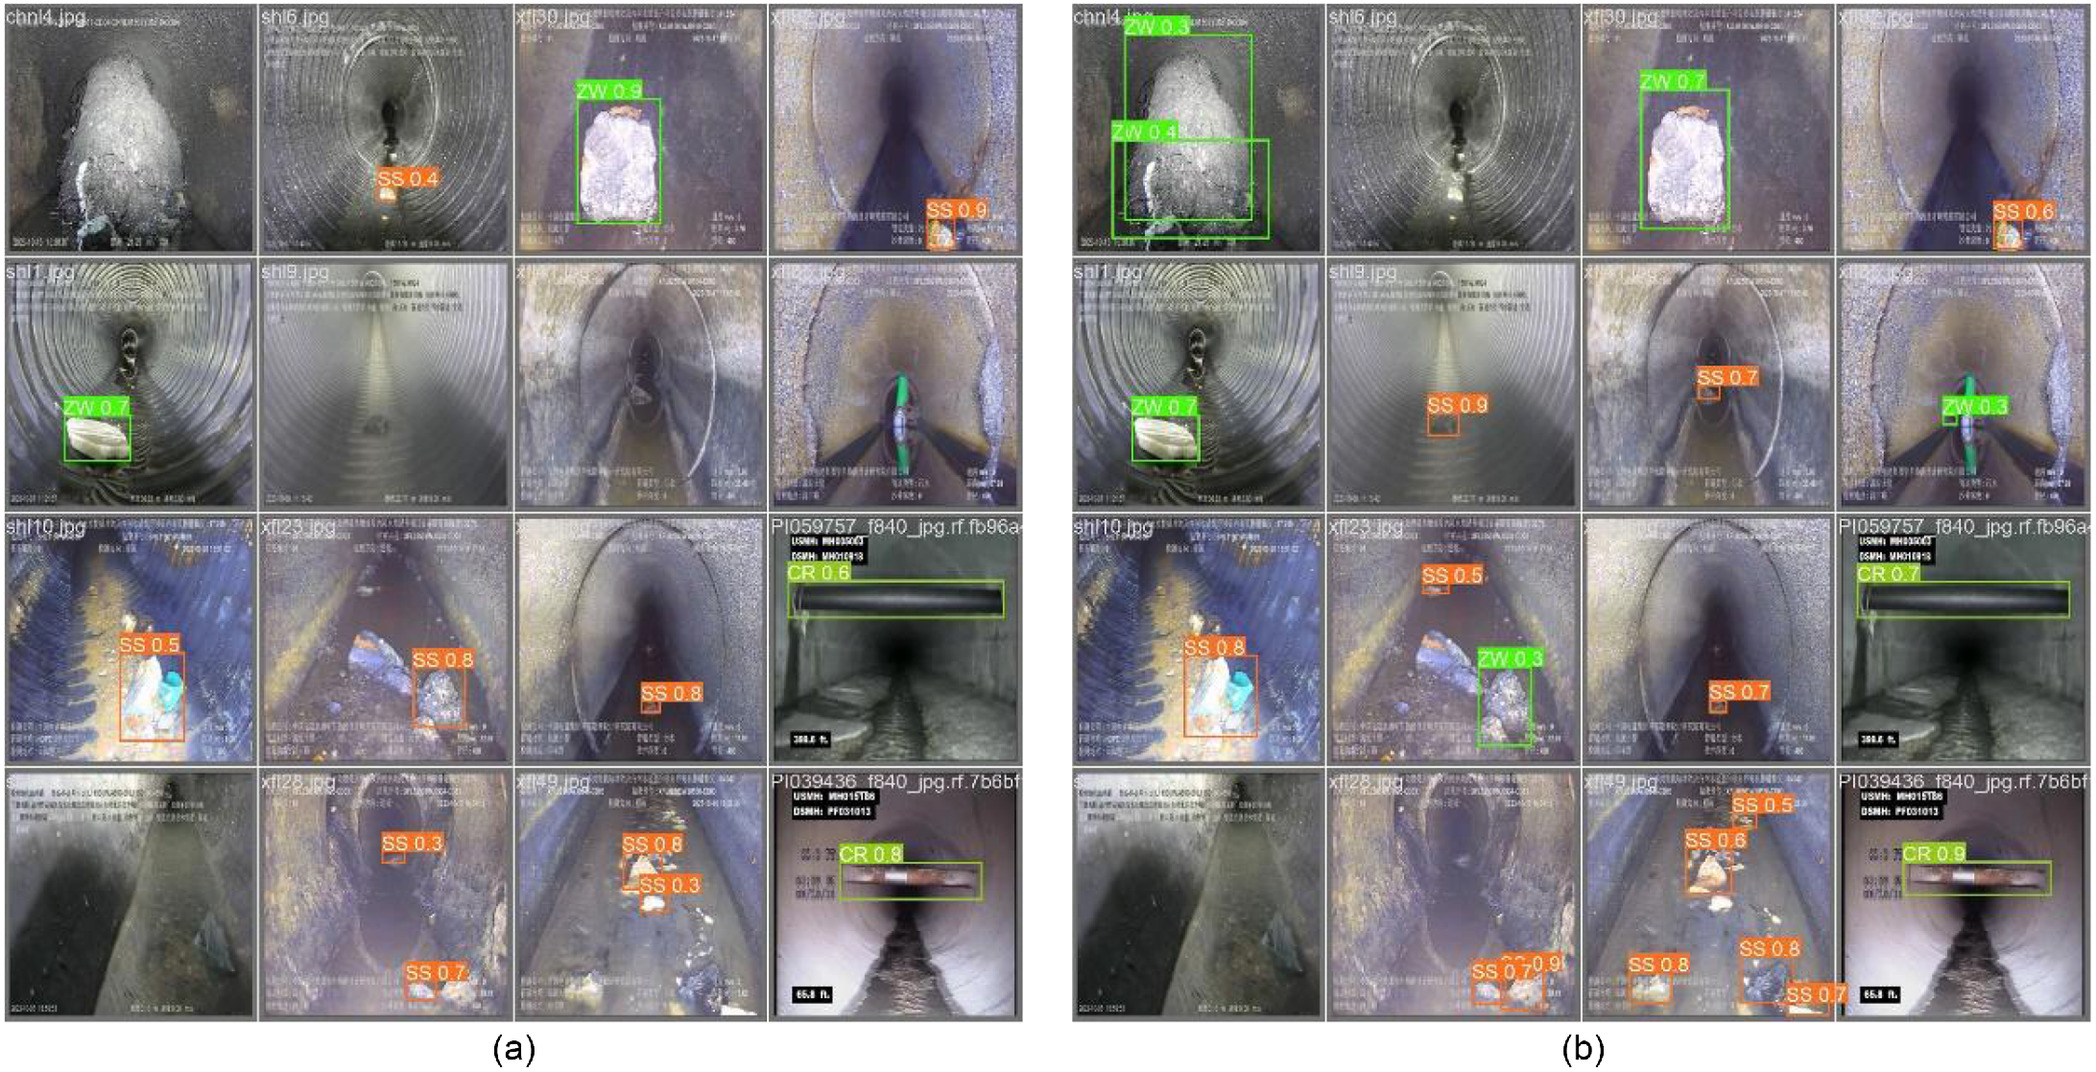
\includegraphics[width=0.8\linewidth]{images/object-detect/yolo5_object_detection.jpg}
    \caption{YOLOv5 for pipeline defects}
\end{figure}
\end{frame}
